\section{Results}
\label{sec:results}
Our experiments address three questions that follow from the toy example in Sec.~\ref{sec:intro}: whether a correctly placed forecast changes the scorer's decisions on held-out data, whether it changes the crop decision or the returned location, and which readout and which insertion conditions realize the effect. We then test whether the effect survives the move to native vessels and to thresholds calibrated on another acquisition.

\begin{figure}[t]
\centering
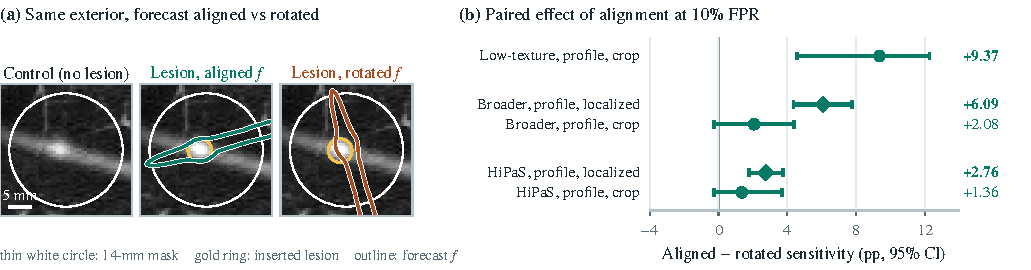
\includegraphics[width=\columnwidth]{figures/placement.pdf}
\caption{The same forecast helps only when it is correctly placed. (a)~Development example with the aligned and rotated forecast outlines; gold ring: inserted lesion; thin circle: 14-mm mask. (b)~Aligned minus rotated sensitivity of the profile readout at the matched 10\% FPR; circles: crop, diamonds: localized sensitivity; bold values exclude zero.}
\label{fig:placement}
\end{figure}

\begin{table}[t]
\centering
\small
% One-column version of tables/decisive.tex (same numbers; revision 7).
\setlength{\tabcolsep}{1.2pt}\footnotesize
\begin{tabular}{@{}lrrr@{\hspace{6pt}}r@{}}
\toprule
& Low-text. & \multicolumn{3}{c}{Broader held-out set} \\
\cmidrule(l){3-5}
Readout & sens. & sens. & loc. sens. & frozen \\
\midrule
\textbf{Fixed, aligned} & \textbf{50.75} & \textbf{24.05} & \textbf{15.38} & \textbf{24.74\,/\,10.59} \\
Fixed, rotated       & 36.03 & 20.81 & 5.72  & 21.18\,/\,10.15 \\
Plug-in, aligned     & 39.45 & 22.54 & 11.54 & 23.86\,/\,10.44 \\
Plug-in, rotated     & 37.39 & 21.26 & 6.92  & 19.81\,/\,9.12 \\
Profile, aligned & 46.50 & 23.32 & 13.45 & 23.79\,/\,10.59 \\
Profile, rotated     & 37.13 & 21.23 & 7.35  & 19.29\,/\,8.82 \\
Prof.\ rot., aligned clf. & -- & 19.26 & 9.19 & 19.20\,/\,10.00 \\
CT + shell           & 36.60 & 21.50 & 13.49 & 21.66\,/\,10.29 \\
CT only              & 32.88 & 21.39 & 13.37 & 23.78\,/\,11.62 \\
Hessian subtr.  & 47.34 & 14.31 & --    & 14.31\,/\,10.29 \\
\midrule
\multicolumn{5}{@{}l}{\emph{Lead minus \ldots\ (pp, 95\% CI)}}\\
$-$ refitted rotation & -- & \multicolumn{1}{r}{$+2.1$} & \multicolumn{1}{r}{$+6.1$} & -- \\
                      &    & \scriptsize[$-0.3,+4.4$] & \scriptsize[$+4.4,+7.8$] & \\
$-$ fixed subtr.     & -- & \multicolumn{1}{r}{$-0.7$} & \multicolumn{1}{r}{$-1.9$} & -- \\
                      &    & \scriptsize[$-3.0,+0.5$] & \scriptsize[$-3.3,-1.0$] & \\
\bottomrule
\end{tabular}

\caption{Sensitivity (\%) at the matched 10\% FPR on the low-texture subset and the broader held-out set, and at the frozen LUNA16 cutoffs (sensitivity\,/\,achieved FPR). Bold: best aligned readout per column. A dash marks a quantity not computed in that setting.}
\label{tab:decisive}
\end{table}

\subsection{Effect of Forecast Alignment}
\label{sec:res_align}
We first ask whether the aligned forecast improves the prespecified scorer on the broader held-out set. Fig.~\ref{fig:placement} summarizes the paired effect of alignment in all three settings, and Table~\ref{tab:decisive} lists every scorer. The broader set is considerably harder than the development data: at the matched 10\% FPR the readouts accept between about 19\% and 24\% of lesion crops, and the Hessian baseline only 14.31\%. The aligned profile increased crop sensitivity by $+2.08\pp$ \ci{-0.27}{+4.40} over the rotation with a refitted classifier and by $+4.05\pp$ \ci{+1.37}{+6.23} over the rotation evaluated with the aligned classifier. At frozen cutoffs the difference was $+4.50\pp$, albeit at achieved FPRs of 10.59\% \vs 8.82\%; including calibration uncertainty, the interval was \ci{-0.59}{+8.31}\,pp and the upper limit on excess FPR $5.00\pp$. The prespecified crop-level criterion was therefore not met. The two controls without a spatial field behave as expected: the CT-only and CT + shell scorers accept 21.39\% and 21.50\% of lesion crops, so exterior summaries alone add essentially nothing. Localization, in contrast, improved substantially (Fig.~\ref{fig:localization}): the rotated profile returned the lesion location for 7.35\% of insertions and the aligned profile for 13.45\%, a gain of $+6.09\pp$ \ci{+4.38}{+7.78}. The same pattern holds for every forecast-conditioned readout: with the rotated forecast, fixed subtraction localizes 5.72\%, the plug-in readout 6.92\% and the profile 7.35\% of insertions, all below the CT-only scorer (13.37\%), whereas with the aligned forecast they reach 15.38\%, 11.54\% and 13.45\%. A misplaced forecast thus localizes worse than no forecast at all, consistent with the toy example: its subtraction removes nothing from the vessel and distorts the background elsewhere.

The low-texture subset, where vessels compete most strongly with the lesion, shows the placement effect already at the crop level. There the aligned profile outperformed its rotation by $+9.66\pp$ \ci{+8.10}{+11.19} at frozen cutoffs (achieved FPR 10.38\% \vs 10.02\%) and by $+9.37\pp$ \ci{+4.56}{+12.29} at matched FPR (Fig.~\ref{fig:placement}b). Under the shared readouts, fixed subtraction gained $+14.72\pp$ \ci{+11.11}{+17.05} over its rotation and $+14.15\pp$ \ci{+10.73}{+16.44} over the CT + shell control, gaining 2,001 and losing 546 positive decisions relative to the rotation (Table~\ref{tab:decisive}). Because these cases informed the design of the readouts, we regard them as supporting rather than confirmatory evidence.

\begin{figure}[t]
\centering
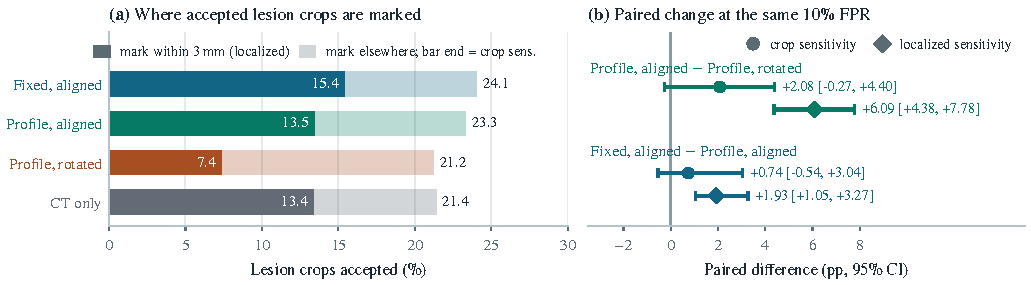
\includegraphics[width=\columnwidth]{figures/localization.pdf}
\caption{Acceptance and localization are distinct decisions (broader held-out set, matched 10\% FPR). (a)~Accepted lesion crops whose returned location lies within 3\,mm of the lesion (dark) or elsewhere (light). (b)~Paired differences with 95\% CIs.}
\label{fig:localization}
\end{figure}

\subsection{Acceptance versus Localization}
\label{sec:res_loc}
A crop-by-crop comparison of the two placements explains the difference between the endpoints. Of the net gain of 746 localized insertions, about a third arises from crops accepted under both placements, where alignment moves the returned location onto the lesion (386 crops, against 124 moved away); the remainder comes from crops that only the aligned profile accepts (647 \vs 163; Table~S3). Localization therefore improves considerably more than acceptance. This behavior follows from the competition illustrated in Fig.~\ref{fig:overview}: if a vessel response $m(x_v)$ exceeds a lesion response $m(x_\ell)$ and conditioning lowers them by $d_v$ and $d_\ell$, the lesion becomes the maximum when $d_v-d_\ell>m(x_v)-m(x_\ell)$, regardless of whether the crop decision changes.

The localization gain does not depend on the choice of readout or on refitting. In a post hoc analysis, fixed subtraction compared with its own separately tuned rotation gains $+9.66\pp$ \ci{+8.24}{+11.38} in localized sensitivity on the broader set and $+2.39\pp$ \ci{+1.22}{+3.28} on HiPaS. Rotating only the field under the aligned classifier yields $+4.26\pp$ \ci{+2.39}{+5.83} and $+0.51\pp$ \ci{-0.15}{+1.09}, respectively.

\subsection{Readout Flexibility and Learned Baselines}
\label{sec:res_gain}
Additional flexibility in the vessel amplitude did not improve performance (Table~\ref{tab:decisive}). On the broader set, the plug-in readout, which re-estimates the gain inside the window without a lesion term, is the weakest aligned readout in both crop (22.54\%) and localized sensitivity (11.54\%). On the low-texture subset, the profile trailed the Hessian baseline by $0.84\pp$ \ci{-6.15}{+2.43}, whereas fixed subtraction exceeded it by $3.41\pp$ \ci{-0.23}{+6.05}. On the broader set, the profile trailed fixed subtraction by $0.74\pp$ \ci{-3.04}{+0.54} in crop sensitivity, and fixed subtraction localized $1.93\pp$ \ci{+1.05}{+3.27} more insertions (15.38\% of all insertions). On 18 development backgrounds with exact fields, where the forecast equals the added vessel, fixed subtraction and profiling both ordered 67.6\% of insertion/control pairs correctly, compared with 62.0\% for the plug-in readout. These results are consistent with the analysis in Sec.~\ref{sec:readout}: a gain estimated inside the core can absorb part of the lesion.

The CT-only CNN reached 67.54\% development AUROC and 36.28\% sensitivity at the 10\% cap, comparable to the ridge classifier on the CT-only readout (68.08\% and 36.47\%). Table~\ref{tab:learned} compares its four second inputs on the low-texture subset: smoothed CT reaches 34.28\% sensitivity, the aligned and rotated forecasts 35.14\% and 35.68\%, and the residual $y-f$ 36.44\%. The aligned-minus-rotated difference was $-0.54\pp$ \ci{-2.80}{+0.62}, and the residual input changed sensitivity by $+2.16\pp$ \ci{-1.19}{+4.44}. The network is not under-trained: it fits small training sets almost perfectly, and its development AUROC increases with the number of fitting patients (Sec.~S6 and Fig.~S1). A classifier that pools learned features can therefore use the same field without exploiting its placement; the placement gain is specific to a readout in which the field can suppress a competing peak.

\begin{table}[t]
\centering
% Learned comparison (moved from supplement; same numbers).
\setlength{\tabcolsep}{3pt}\footnotesize
\begin{tabular}{@{}lrrrr@{}}
\toprule
Second input & Epoch & Dev.\ AUROC & AUROC & Sens. \\
\midrule
Smoothed CT & 30 & 67.54 & 68.78 & 34.28 \\
Aligned forecast & 20 & 67.54 & 68.81 & 35.14 \\
Rotated forecast & 30 & 67.81 & 69.13 & 35.68 \\
Residual $y-f$ & 30 & 68.16 & 69.46 & 36.44 \\
\bottomrule
\end{tabular}

\caption{Hybrid CNN with four second inputs on the low-texture subset (\%), with identical architecture, data, seeds and budget. The ridge classifier on the CT-only readout reaches 69.17\% AUROC and 32.88\% sensitivity.}
\label{tab:learned}
\end{table}


\subsection{Analysis by Insertion Condition}
\label{sec:conditions}
Fig.~\ref{fig:strata} decomposes the paired crop-level gain by insertion condition, evaluated at each setting's global cutoff. Gains concentrate where a vessel is most likely to produce the search maximum, namely for displaced, high-contrast insertions, which gained $+15.40\pp$ \ci{+11.84}{+19.08} on the broader set. Centered insertions changed by $-5.34\pp$ \ci{-9.49}{-1.25} and the faintest insertions by $-1.47\pp$ \ci{-2.60}{-0.24}, while insertions overlapping a vessel by at least 50\% were unaffected ($-0.12\pp$ \ci{-3.59}{+3.23}). A centered lesion is often already the strongest response, and a faint lesion leaves a weak residual even when the vessel is well explained. The low-texture subset exhibits the same pattern with larger effects.

We also evaluated a forecast-dominance score that is available before scoring, defined as the peak forecast relative to the texture of the shell (Sec.~S5). Crops in the upper half of this score, 40.7\% of the broader set, show a gain of $+3.29\pp$ \ci{+0.04}{+6.03}, but the high-minus-low interaction of $+2.03\pp$ \ci{-1.62}{+5.11} is not resolved. Within the high-dominance band, alignment also raises the frozen FPR (11.19\% \vs 9.39\%; Sec.~S5), so the score describes where alignment matters but does not by itself identify a better operating point.

\begin{figure}[t]
\centering
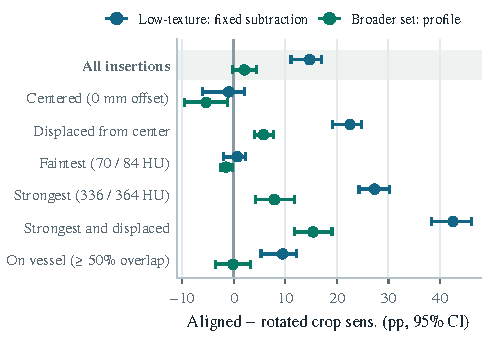
\includegraphics[width=\columnwidth]{figures/strata.pdf}
\caption{Placement gains by insertion condition: aligned minus rotated crop sensitivity at each setting's 10\% FPR cap, for fixed subtraction on the low-texture subset and the profile on the broader set. Rows are not mutually exclusive.}
\label{fig:strata}
\end{figure}

\subsection{Transfer to Native Vessels}
\label{sec:native}
On the 72 HiPaS scans, 7,713 of the 7,776 insertions lie within 2\,mm of an annotated artery or vein. At matched FPR, alignment improved localized sensitivity by $+2.76\pp$ \ci{+1.77}{+3.76} and crop sensitivity by $+1.36\pp$ \ci{-0.26}{+3.69}. The localization gain therefore persists when real anatomy, including curved vessels that a straight chord approximates poorly, supplies the competing response. Table~\ref{tab:hipas} lists all scorers. Fixed subtraction (5.66\%), the profile (5.47\%) and the plug-in readout (5.31\%) localize roughly twice as many insertions as their rotations (3.27\%, 2.70\% and 2.84\%), and more than the CT-only (3.38\%) and CT + shell (4.21\%) scorers; alignment produced 284 newly localized insertions against 69 lost. At the crop level, all scorers accept 14--16\% of lesion crops except the Hessian baseline (11.33\%).

\begin{table}[t]
\centering
% One-column version of tables/transfer.tex (same numbers; revision 7).
\setlength{\tabcolsep}{3pt}\footnotesize
\begin{tabular}{@{}lrrr@{}}
\toprule
& \multicolumn{2}{c}{Matched 10\% FPR} & LUNA16 cutoffs \\
\cmidrule(lr){2-3}\cmidrule(l){4-4}
Readout & sens. & loc.\ sens. & sens.\,/\,FPR \\
\midrule
CT only              & 14.47 & 3.38 & 10.83\,/\,7.87 \\
CT + shell           & 14.45 & 4.21 & 4.69\,/\,2.55 \\
Hessian subtraction  & 11.33 & --   & 12.04\,/\,10.88 \\
Fixed, aligned       & 16.26 & 5.66 & 1.93\,/\,0.46 \\
Fixed, rotated       & 14.30 & 3.27 & 5.00\,/\,2.55 \\
Plug-in, aligned     & 15.64 & 5.31 & 2.31\,/\,0.69 \\
Plug-in, rotated     & 14.63 & 2.84 & 6.53\,/\,3.94 \\
\textbf{Profile, aligned} & \textbf{15.52} & \textbf{5.47} & \textbf{2.15\,/\,0.69} \\
Profile, rotated     & 14.16 & 2.70 & 6.62\,/\,4.63 \\
Profile, rot., aligned clf. & 14.97 & 4.95 & 0.91\,/\,0.23 \\
\bottomrule
\end{tabular}

\caption{Sensitivity (\%) on HiPaS native vessels (432 controls, 7,776 insertions) at the within-HiPaS 10\% FPR cap and at the frozen LUNA16 cutoffs.}
\label{tab:hipas}
\end{table}


\subsection{Ranking versus Calibration}
\label{sec:calibration}
When applied unchanged to HiPaS, the LUNA16 cutoffs yielded 2.15\% sensitivity at 0.69\% FPR for the aligned profile, compared with 6.62\% at 4.63\% for its rotation (Table~\ref{tab:hipas} and Fig.~\ref{fig:roc}b). Most scorers accepted far fewer HiPaS controls than the nominal 10\%, so their realized operating points shifted. Fig.~\ref{fig:roc} shows the ROC curves underlying these operating points, computed with the negatives of each cohort. On the broader set, both aligned readouts lie above the rotation and the CT-only scorer between approximately 3\% and 25\% FPR, so the matched result does not depend on the choice of a 10\% cap. On HiPaS the crop-level curves nearly coincide, and the gain is confined to localization. The frozen LUNA16 cutoffs (open circles) fall close to the 10\% cap on LUNA16 but far below it on HiPaS. Table~\ref{tab:cal} quantifies the contribution of calibration uncertainty: resampling the 175 calibration patients widens the broader lead-minus-rotation interval from $[+2.62,+6.32]$ to $[-0.59,+8.31]\pp$. On HiPaS the lead scorer accepts fewer insertions and fewer controls than its rotation, which reflects a shift of the operating point rather than a loss in ranking (Table~\ref{tab:hipas}).

\paragraph{Transfer conditions of the low-texture design.}
The same distinction appears in two additional transfer conditions of the low-texture design, a LUNA16 morphology shift and an independent LNDb acquisition with shifted insertions~\cite{pedrosa2021}. Neither met its full transfer criteria at frozen cutoffs (Table~\ref{tab:old}); on the low-texture subset itself, the upper limit on excess FPR relative to the CT-only scorer was $4.92\pp$ against a prespecified 4\,pp. Within each test set, however, the profile and Hessian sensitivities at 10\% FPR were 37.93\% and 37.44\% under the morphology shift and 33.15\% and 32.94\% on LNDb, so ranking transferred better than the cutoffs. On LNDb, adding the spatial features to the scores of a published detector changed mean FROC by $0.00\pp$ \ci{-0.21}{+0.23} relative to the full CT-only classifier and by $-0.13\pp$ \ci{-0.33}{+0.35} relative to the sham.

\begin{table}[t]
\centering
% One-column version of tables/calibration.tex (same numbers; revision 7).
\setlength{\tabcolsep}{1.5pt}\footnotesize
\begin{tabular}{@{}llrr@{}}
\toprule
Contrast & Intervals & Sensitivity $\Delta$ & FPR $\Delta$ \\
\midrule
\multicolumn{4}{@{}l}{\emph{Broader LUNA16}}\\
Lead$-$rot. & frozen  & $+4.50$ [$+2.62,+6.32$] & $+1.76$ [$-0.59,+4.12$] \\
                  & recal.  & $+4.50$ [$-0.59,+8.31$] & $+1.76$ [$-2.35,+5.00$] \\
Lead$-$fixed & frozen  & $-0.95$ [$-1.85,-0.10$] & $+0.00$ [$-1.32,+1.32$] \\
                  & recal.  & $-0.95$ [$-3.80,+1.32$] & $+0.00$ [$-2.21,+1.76$] \\
\multicolumn{4}{@{}l}{\emph{HiPaS}}\\
Lead$-$rot. & frozen  & $-4.48$ [$-6.51,-2.58$] & $-3.94$ [$-6.02,-2.08$] \\
                  & recal.  & $-4.48$ [$-7.09,-2.60$] & $-3.94$ [$-6.02,-1.62$] \\
Lead$-$fixed & frozen  & $+0.22$ [$-0.05,+0.62$] & $+0.23$ [$+0.00,+0.69$] \\
                  & recal.  & $+0.22$ [$-0.32,+0.73$] & $+0.23$ [$+0.00,+0.69$] \\
\bottomrule
\end{tabular}

\caption{Paired differences of the aligned profile at the frozen LUNA16 cutoffs (pp, 95\% CI), with intervals conditional on the calibration set (frozen) or resampling it (recal.).}
\label{tab:cal}
\end{table}

\begin{table}[t]
\centering
% Original frozen operating points (moved from supplement; same numbers).
\setlength{\tabcolsep}{2.5pt}\footnotesize
\begin{tabular}{@{}lrrrrrr@{}}
\toprule
& \multicolumn{2}{c}{Profile} & \multicolumn{2}{c}{Rotation} & \multicolumn{2}{c}{Hessian} \\
\cmidrule(lr){2-3}\cmidrule(lr){4-5}\cmidrule(l){6-7}
Condition & Sens. & FPR & Sens. & FPR & Sens. & FPR \\
\midrule
Low-texture subset & 46.85 & 10.38 & 37.19 & 10.02 & 38.39 & 5.46 \\
Morphology shift & 41.79 & 12.05 & 32.69 & 9.24 & 32.06 & 6.43 \\
LNDb + morphology & 28.04 & 6.49 & 29.27 & 9.14 & 36.09 & 12.09 \\
\bottomrule
\end{tabular}

\caption{Frozen operating points (\%) of the low-texture design on the subset itself and two transfer conditions, using its own 276 calibration negatives.}
\label{tab:old}
\end{table}

\begin{figure}[t]
\centering
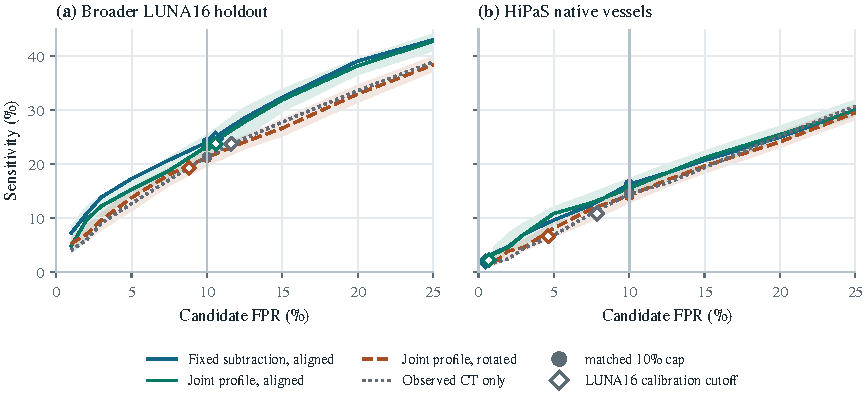
\includegraphics[width=\columnwidth]{figures/roc.pdf}
\caption{ROC curves with pointwise 95\% bands for the profile placements; open circles mark the frozen LUNA16 cutoffs, which transfer poorly to HiPaS.}
\label{fig:roc}
\end{figure}
